% Template for Elsevier CRC journal article
% version 1.2 dated 17 May 2021

% This file (c) 2009-2021 Elsevier Ltd.  Modifications may be freely made,
% provided the edited file is saved under a different name

% This file contains modifications for Transportation Research Procedia

% Changes since version 1.1
% - added "procedia" option compliant with ecrc.sty version 1.2a
%   (makes the layout approximately the same as the Word CRC template)
% - added example for generating copyright line in abstract

%-----------------------------------------------------------------------------------

%% This template uses the elsarticle.cls document class and the extension package ecrc.sty
%% For full documentation on usage of elsarticle.cls, consult the documentation "elsdoc.pdf"
%% Further resources available at http://www.elsevier.com/latex

%-----------------------------------------------------------------------------------

%%%%%%%%%%%%%%%%%%%%%%%%%%%%%%%%%%%%%%%%%%%%%%%%%%%%%%%%%%%%%%
%%%%%%%%%%%%%%%%%%%%%%%%%%%%%%%%%%%%%%%%%%%%%%%%%%%%%%%%%%%%%%
%%                                                          %%
%% Important note on usage                                  %%
%% -----------------------                                  %%
%% This file should normally be compiled with PDFLaTeX      %%
%% Using standard LaTeX should work but may produce clashes %%
%%                                                          %%
%%%%%%%%%%%%%%%%%%%%%%%%%%%%%%%%%%%%%%%%%%%%%%%%%%%%%%%%%%%%%%
%%%%%%%%%%%%%%%%%%%%%%%%%%%%%%%%%%%%%%%%%%%%%%%%%%%%%%%%%%%%%%

%% The ’3p’ and ’times’ class options of elsarticle are used for Elsevier CRC
%% The ’procedia’ option causes ecrc to approximate to the Word template
\documentclass[5p,times,procedia]{elsarticle}
\flushbottom

%% The `ecrc’ package must be called to make the CRC functionality available
\usepackage{ecrc}
%\usepackage{amsmath}


%% The ecrc package defines commands needed for running heads and logos.
%% For running heads, you can set the journal name, the volume, the starting page and the authors

%% set the volume if you know. Otherwise `00’
\volume{00}

%% set the starting page if not 1
\firstpage{1}

%% Give the name of the journal
\journalname{Procedia CIRP}

%% Give the author list to appear in the running head
%% Example \runauth{C.V. Radhakrishnan et al.}
\runauth{B. Bertschinger et al.}

%% The choice of journal logo is determined by the \jid and \jnltitlelogo commands.
%% A user-supplied logo with the name <\jid>logo.pdf will be inserted if present.
%% e.g. if \jid{yspmi} the system will look for a file yspmilogo.pdf
%% Otherwise the content of \jnltitlelogo will be set between horizontal lines as a default logo

%% Give the abbreviation of the Journal.
\jid{trpro}

%% Give a short journal name for the dummy logo (if needed)
%\jnltitlelogo{Transportation Research}

%% Hereafter the template follows `elsarticle’.
%% For more details see the existing template files elsarticle-template-harv.tex and elsarticle-template-num.tex.

%% Elsevier CRC generally uses a numbered reference style
%% For this, the conventions of elsarticle-template-num.tex should be followed (included below)
%% If using BibTeX, use the style file elsarticle-num.bst

%% End of ecrc-specific commands
%%%%%%%%%%%%%%%%%%%%%%%%%%%%%%%%%%%%%%%%%%%%%%%%%%%%%%%%%%%%%%%%%%%%%%%%%%

%% The amssymb package provides various useful mathematical symbols

\usepackage{amssymb}
%% The amsthm package provides extended theorem environments
%% \usepackage{amsthm}

%% The lineno packages adds line numbers. Start line numbering with
%% \begin{linenumbers}, end it with \end{linenumbers}. Or switch it on
%% for the whole article with \linenumbers after \end{frontmatter}.
%% \usepackage{lineno}

%% natbib.sty is loaded by default. However, natbib options can be
%% provided with \biboptions{...} command. Following options are
%% valid:

%%   round  -  round parentheses are used (default)
%%   square -  square brackets are used   [option]
%%   curly  -  curly braces are used      {option}
%%   angle  -  angle brackets are used    <option>
%%   semicolon  -  multiple citations separated by semi-colon
%%   colon  - same as semicolon, an earlier confusion
%%   comma  -  separated by comma
%%   numbers-  selects numerical citations
%%   super  -  numerical citations as superscripts
%%   sort   -  sorts multiple citations according to order in ref. list
%%   sort&compress   -  like sort, but also compresses numerical citations
%%   compress - compresses without sorting
%%
%\biboptions{authoryear}

% \biboptions{}

% if you have landscape tables
\usepackage[figuresright]{rotating}
%\usepackage{harvard}
% put your own definitions here:x
%   \newcommand{\cZ}{\cal{Z}}
%   \newtheorem{def}{Definition}[section]
%   ...

% add words to TeX’s hyphenation exception list
%\hyphenation{author another created financial paper re-commend-ed Post-Script}

% declarations for front matter

\usepackage[bookmarks=false]{hyperref}
\hypersetup{colorlinks,
linkcolor=blue,
citecolor=blue,
urlcolor=blue}

\usepackage{enumitem}
\usepackage{amsmath}
\usepackage{subcaption}
%\usepackage{kbordermatrix}
\usepackage{tikz}
\usepackage{relsize}
\usepackage{lipsum}

\AtBeginDocument{%
\addtolength\abovedisplayskip{-1.5\baselineskip}%
\addtolength\belowdisplayskip{-1.0\baselineskip}%
\addtolength\abovedisplayshortskip{-2.0\baselineskip}%
\addtolength\belowdisplayshortskip{-1.0\baselineskip}%
}

% figures
\usepackage{tikz}
\usepackage{tikzscale}
\usepackage{pgf}
\usepackage{pgfplots}
\usepackage{pgfplotstable}
\pgfplotsset{compat=newest}

\usetikzlibrary{calc,
	%	external,
	pgfplots.units,
	%	pgfplots.external,
	pgfplots.groupplots,
	arrows,
	intersections,
	patterns,
	positioning,
	shapes,
	plotmarks,
	decorations.pathmorphing,
	decorations.markings
}

\begin{document}
\begin{frontmatter}
	
	%% Title, authors and addresses
	
	%% use the tnoteref command within \title for footnotes;
	%% use the tnotetext command for the associated footnote;
	%% use the fnref command within \author or \address for footnotes;
	%% use the fntext command for the associated footnote;
	%% use the corref command within \author for corresponding author footnotes;
	%% use the cortext command for the associated footnote;
	%% use the ead command for the email address,
	%% and the form \ead[url] for the home page:
	%%
	%% \title{Title\tnoteref{label1}}
	%% \tnotetext[label1]{}
	%% \author{Name\corref{cor1}\fnref{label2}}
	%% \ead{email address}
	%% \ead[url]{home page}
	%% \fntext[label2]{}
	%% \cortext[cor1]{}
	%% \address{Address\fnref{label3}}
	%% \fntext[label3]{}
	
	\dochead{18th CIRP Conference on Intelligent Computation in Manufacturing Engineering}%
	
	\title{A new Software Driven External Sensor System for Industrial Robots}
	
	%% use optional labels to link authors explicitly to addresses:
	%% \author[label1,label2]{<author name>}
	%% \address[label1]{<address>}
	%% \address[label2]{<address>}
	
	\author[a]{Bernd Bertschinger\corref{*}}
	\author[b]{Kathrin Hoffmann}
	\author[c]{Jan Baumgärtner}
	\author[b]{Gajanan Kanagalingam}
	\author[c]{Jürgen Fleischer}
	\author[b]{Oliver Sawodny}
	\author[a]{Stephan Reichelt}
	%\ead{author@institute.xxx}
	
	\address[a]{Institute of Applied Optics, University of Stuttgart - ITO, Pfaffenwaldring 9, 70569 Stuttgart, Germany}
	\address[b]{Institute for System Dynamics, University of Stuttgart - ISYS, Waldburgstr. 17/19, 70563 Stuttgart, Germany}
	\address[c]{Institute of Production Science, Karlsruhe Institute of Technology - WBK, Kaiserstraße 12, 76131 Karlsruhe, Germany}
	
	\aucores{* Bernd Bertschinger, Tel.: +49-711-685-69892. {\it E-mail address:} bernd.bertschinger@ito.uni-stuttgart.de}
	
	\begin{abstract}
		%% Text of abstract
		For decades, laser tracker and working station have been the state of the art to measure externally the position disturbances in robotic systems. High system costs limit their usage for control systems in common production machines. We present details for an alternative software-driven approach. Hereby, we combine a new self-referencing, high-precision photogrammetry sensor system with a software for camera placement layout and trajectory optimization. Furthermore, we outline the integration in a closed loop control system and corresponding strategies.
	\end{abstract}
	
	\begin{keyword}
		Type your keywords here, separated by semicolons ;
		
		%% keywords here, in the form: keyword \sep keyword
		
		%% PACS codes here, in the form: \PACS code \sep code
		
		%% MSC codes here, in the form: \MSC code \sep code
		%% or \MSC[2008] code \sep code (2000 is the default)
		
	\end{keyword}
	%\cortext[cor1]{Corresponding author. Tel.: +0-000-000-0000 ; fax: +0-000-000-0000.}
	
\end{frontmatter}

%%
%% Start line numbering here if you want
%%
% \linenumbers

%% main text

\section{Introduction}

%motivation: industrial robots instead of specialized machinery, adaptable to various tasks in manufacturing, low cost \\
%limiting factor: accuracy of robot
%
%approach: software-defined planning of the robot configuration, path and trajectory
%
%result: robot motion which is the optimal solution for production precision
%
%setup: (close to?) real-time capable optical measurement system, optical markers attached to robot endeffector
%
%Relevant Errors-Model for Process Perception - Metrological Error \\
%Relevant Errors-Model for Process Planing - Dynamic Error \\
%
%System Setup

Social and ecological changes, as well as the need for
highly individualized and diversified product ranges
motivate not only to increase the efficiency of the means
of production, but also their flexibility of application.
This is addressed by the concept of Wertstromkinematik \textit{Referenz etc.}.
Herein the factory is not a static setup to produce
one set of goods, but can be dynamically reconfigured to be a generalized production floor.\\
To become a valid means of production, the system needs not only to
be more productive, but also as flexible and cost-efficient as possible. This need for flexibility in turn leads to an increase of precision, which can be used to either facilitate the production of high-precision components, for human-robot and robot-robot collaboration, as well as a trade-off for higher process speed.\\
By the current state of technology this is a dilemma, because state of the art detection system use internal sensor, which require an exceeding level of mechanical stiffness, which in turn leads to high
acquisition costs. An alternative to internal sensor system are external sensors, such laser trackers and tracking stations. The costs of these systems make them unsuitable for wide-spread production applications, but are rather used as means for calibration.\\

\textcolor{red}{literature on system with laser tracker? }%literature review: with laser tracker: e.\,g.~\cite{Moeller17, Yang17}

\subsection{Scope of this Paper}

Instead a holistic approach is needed, which combines in a software driven approach the placement and configuration of the sensor system with the trajectory generation in consideration of the kinematic control properties.s

\lipsum[1-1]

%\vspace*{2pt}
%\renewcommand{\labelenumii}{\theenumii}
%\renewcommand{\theenumii}{\theenumi.\arabic{enumii}.}
%\vspace*{8pt}
%\setlist{nolistsep}

\section{Process Perception}

Recent research indicates that multipoint photogrammetry might be a solution to realize cost-efficient high-resolution optical sensors \cite{Hartlieb_2021}.
The schematics of this measuring method is shown in Fig.~\ref{fig:MeasSys_Errors}.
\begin{figure}[h]
	\centering
	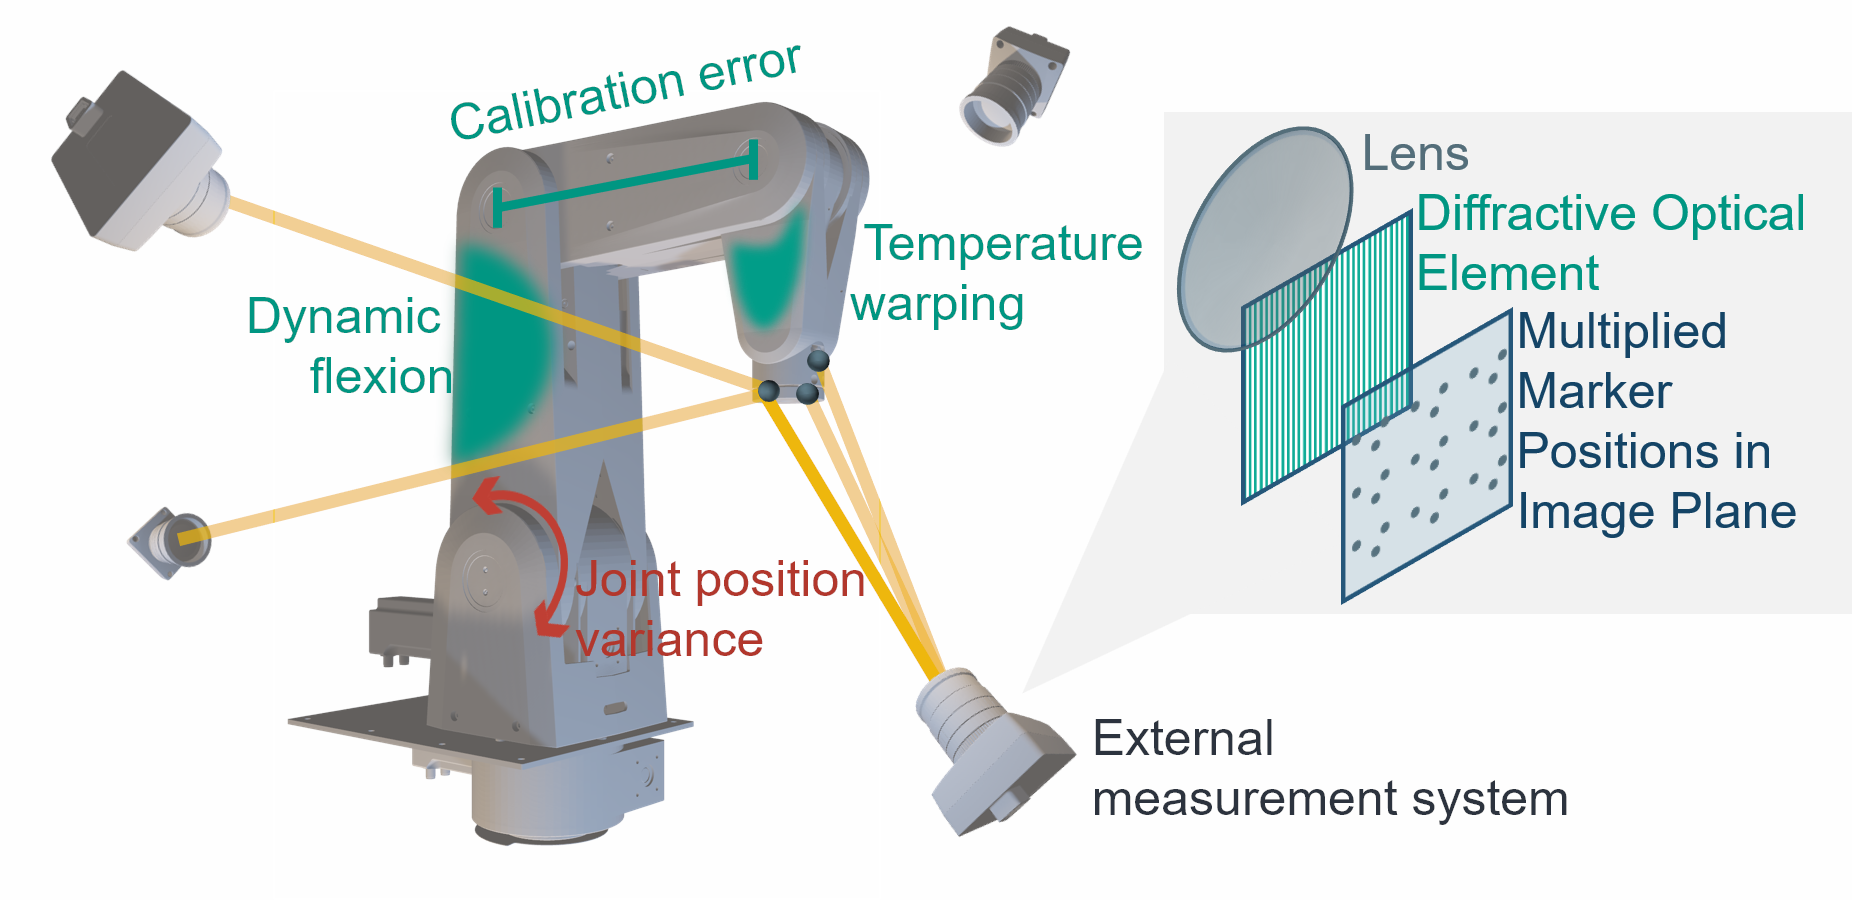
\includegraphics[width=\columnwidth]{graphics/error_sources.png}
	\caption{Error sources in a robotic manufacturing system, which can be compensated using an external multipoint  sensor are marked in green.}
	\label{fig:MeasSys_Errors}
\end{figure}
In this method, as can be seen in Fig.~\ref{fig:error_sources}, a Diffractive Optical Element (DOE) is used in succession of an imaging lens to create multiple linearly independent optical copies of an active marker.
It has been shown [\textcolor{red}{add reference here}] that the variance of the mean positional detection error of these points $\sigma_{x’y’}$ detected on the imaging sensor is proportional to the number of copies $n_pt$ created by the DOE.
\begin{equation}
	\textcolor{red}{\sigma_{x’y’}^2 = n_{pt}^{}}
\end{equation}
However, this increase in planar signal detection is in itself not sufficient for high precision 3D localization. One or more additional sensors is needed to triangulate the 2D point positions on the imaging sensors to it’s point of origin in the object space. \\
For a pinhole camera system the relation between object and imaging point is determined by the camera Matrix $\mathbf{C}$, which is composed of the intrinsic $\mathbf{K}$ and  and extrinsic camera parameters $[\mathbf{R}, t]$, which comprise information about the spatial orientation, as well as the information about focal width and
image scale factor. This leads to the well established collinear equation \cite{Luhmann2003}, whereby $l_n$ is the collinear factor, which describes the line of sight between the object and image point.

\begin{align}
	\mathbf{C} = \mathbf{K}
	\begin{bmatrix}
		\mathbf{R} & \hat{t} \\
		0 & 1 \\
	\end{bmatrix} \\
	l_{n}
	\begin{bmatrix}
		x_n’ \\
		y_n’ \\
		0
	\end{bmatrix}
	= \mathbf{C}
	\begin{bmatrix}
		x \\
		y \\
		z \\
		0
	\end{bmatrix}
\end{align}
\textcolor{red}{warum tHat?}
Subsequently the correspondance between object position an image points, known as triangulation, can be defined for multiple cameras according to:

%https://cookierobotics.com/007/
\begin{equation}
	\label{eqn:triangulation}
	\begin{bmatrix}
		x_{1}’ \mathbf{C}_{3,1}^{\top} - \mathbf{C}_{1,1}^{\top}\\
		y_{1}’ \mathbf{C}_{3,1}^{\top} - \mathbf{C}_{2,1}^{\top}\\
		x_{2}’ \mathbf{C}_{3,2}^{\top} - \mathbf{C}_{1,2}^{\top}\\
		y_{2}’ \mathbf{C}_{3,2}^{\top} - \mathbf{C}_{2,2}^{\top}\\
		\vdots \\
		x_{n}’ \mathbf{C}_{3,n}^{\top} - \mathbf{C}_{1,n}^{\top}\\
		y_{n}’ \mathbf{C}_{3,n}^{\top} - \mathbf{C}_{2,n}^{\top}\\
	\end{bmatrix}
	\begin{bmatrix}
		x \\
		y \\
		z \\
		1
	\end{bmatrix}
	=
	\begin{bmatrix}
		0 \\
		\vdots \\
		0
	\end{bmatrix},
\end{equation}
where $C_{m,n}$ corresponds to the $m$-th row of the $n$-th camera matrix.
In case the extrinsic and intrinsic camera parameters are fully known, the equation system can be solved by least-square techniques \cite{Ahn2004}.

Whereby $C_{m,n}$ corresponds to the m-th row of the n-th camera Matrix.
In case the extrinsic and intrinsic camera parameters are fully known, the system can be solved by the least-square techniques \cite{Ahn2004}.

It is important to note that this relationship can also be described as by the notation for projective reconstruction \cite{Hartley2018}:
\begin{equation}
	\label{eqn:ProjectiveReconstruction}
	x’^{\top}\mathbf{F}x
\end{equation}
<<<<<<< .mine
Here the fundamental matrix $\mathbf{F}$ is a 3x3 Tensor, which scales in rank according to the number of cameras in the system. Due to the increasing complexity and computing effort, this method is usually constraint to three cameras systems.\\
Instead of a Tensor representation the triangulation relation (\ref{eqn:triangulation}) is stated in implicit form:

=======
Here the fundamental matrix $\mathbf{F}$ is a $3\times 3$ tensor, which scales in rank according to the number of cameras in the system. Due to the increasing complexity and computing effort, this method is usually constraint to three cameras systems.\\
Instead of a Tensor representation the triangulation relation (\ref{eqn:triangulation}) is stated in implicit form

>>>>>>> .theirs
\begin{equation}
	\label{eqn:ImplicitFrom}
	\begin{aligned}
		& g(\mathbf{Q},\mathbf{M}) \\
		& \mathbf{Q} = [\mathbf{P},\mathbf{C}]^{\top}.
	\end{aligned}
\end{equation}

The vector of the input Quantities $\mathbf{Q} = \left[q_1,\dots, q_{n}\right]^{\top}$ is composed of the vector of image points $\mathbf{P} = [x’_1,y’_1, \dots ,x’_n,y’_n]^{\top}$ and the vector of camera parameters, $\mathbf{C} = \left[ \mathbf{C}_1 , \dots , \mathbf{C}_n \right]^{\top}$, which in turn define the object point coordinates $\mathbf{M} =  [x,y,z]^{\top}$ in Cartesian form. \\
The uncertainty of the output $\mathbf{M}$ can be approximated by the 1st order Taylor series with regards to input parameters:

\begin{equation}
	\sigma^2 = \sum_{i=1}^{n}\sum_{j=1}^{n} \left(\frac{\delta g}{\delta q_i}\right) \left(\frac{\delta g}{\delta q_j}\right) \mathrm{cov}(q_i, q_j) 
\end{equation}
where $\mathrm{cov}(q_i, q_j) $ is the covariance between two input parameters. More commonly it is known in the form~\cite{Cox2006}  
\begin{equation}
	\sigma^2 = \mathbf{J_{Q}}\mathbf{\Lambda_{Q}}\mathbf{J_{Q}}^{\top}.
\end{equation}
$\mathbf{J_{Q}}$ is known as design or Jacobi matrix of the partial derivatives of $f$ \textcolor{red}{was ist f} with respect to the input quantities $\mathbf{Q}$, and $\mathbf{\Lambda_Q}$ is the covariance matrix of said input values. \\
The uncertainty of the input parameters is directly tied to the uncertainty of the output parameters
\begin{equation}
	\mathbf{J_{M}}\mathbf{\Lambda_{M}}\mathbf{J_{M}}^{\top} = \mathbf{J_{Q}}\mathbf{\Lambda_{Q}}\mathbf{J_{Q}}^{\top}
\end{equation}
Therein, $\mathbf{J_{M}}$ is the Jacobi matrix of the partial derivatives \textcolor{red}{of what with respect to what} and $\mathbf{\Lambda_{M}}$ is the covariance matrix with respect to the output quantities $\hat{\mathbf{M}}$.
\textcolor{red}{was ist Hat?}
The matrix $\mathbf{\Lambda_{M}}$ is computed as
\begin{equation}
	\mathbf{\Lambda_{M}} = \mathbf{J_{M}^{\Delta}} \left( \mathbf{J_{Q}}\mathbf{\Lambda_{Q}}\mathbf{J_{Q}}^{\top}\right) \left(\mathbf{J_{M}^{\Delta}}\right)^{\top}
\end{equation}
with $ \mathbf{J_{M}^{\Delta}} = \left( \mathbf{J_{M}^{\top}} \mathbf{J_{M}^{}} \right)^{-1}\mathbf{J_{M}^{\top}}$ being the Moore-Penrose pseudo inverse matrix of $\mathbf{J_M}$.

\subsection{Metrological Error}
\label{error_estimate}

The design matrices for the input $\mathbf{J}_{Q}$ and output quantities $\mathbf{J}_{M}$ can be established by a various calibration processes \textcolor{red}{here sources}. Usually a series of known markers is placed in the object space \cite{Luhmann2003}. In case of arbitrary camera positions the minimum number of marker needed corresponds to
\begin{equation}
	\label{eqn:NumCalibPoints}
	\begin{aligned}
		& 	u = u_n \cdot n_{pictures} + u_p \cdot n_{points} + u_k \cdot n_{cameras} \\
		& \text{with: } u_n = 6\text{, } u_p = 3\text{, } u_k = 6 
	\end{aligned}
\end{equation}
\textcolor{red}{Variablen einführen}
It becomes evident, that an increase in the number of cameras $n_{\text{cameras}}$ leads to increasing requirements for the means of calibration (\ref{eqn:NumCalibPoints}) and computational complexity, signified by the increasing rank of the fundamental matrix (\ref{eqn:ProjectiveReconstruction}). Conversely it becomes difficult to determine the metrological error of such as system.\\

It becomes self-evident, that an increase in cameras leads to increasing requirements for the means of calibration (\ref{eqn:NumCalibPoints}) and computational complexity, signified by the increasing rank of the fundamental matrix (\ref{eqn:ProjectiveReconstruction}). Conversly it becomes extinsively difficult to determine the metrological error 
of such as system.\\

\begin{figure}[h]
	\centering
	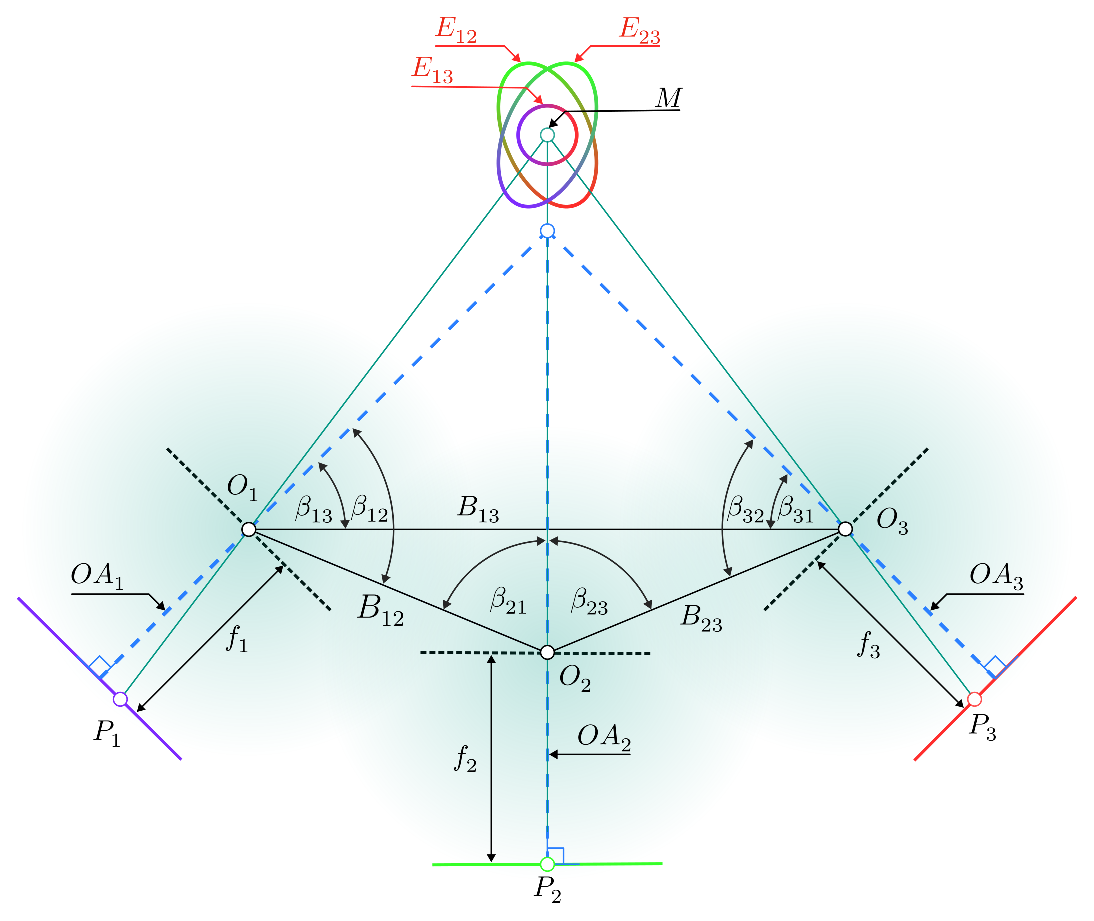
\includegraphics[width=0.8\linewidth]{graphics/MixedErrorCuttingGeometry.eps}
	\caption{Top-Down view on a photogrammetric sensor in tricfocal configuration under simplified converging geometric constraints, whereby the optical axes $OA$ of three cameras systems intersect in one point.		
	It can also be regarded as as composition of $n_{sub}=3$ stereoscopic subsystems, whereby the measurement error of each subsystem corresponds in shape to an ellipsoid $\mathbf{E}$.}
	\label{fig:sub_sensors}
\end{figure}

Hence an alternative approach is needed. As it is depicted in  Fig.~\ref{fig:sub_sensors} a photogrammetric sensor can also be described as a combination of multiple independent stereoscopic sub-sensors.

\begin{equation}
	\label{eqn:CovarianceMatrix}
	n_{sub} = \sum_{n=1}^{n_{cam}}n-1
\end{equation}

For these subsensors the metrological error can be described as an ellipsoid $\mathbf{E}$ \cite{Luhmann2003}, which can be related to spectral decomposition of the covariance of the output quantities $\mathbf{\Lambda_{M}}$.

\begin{equation}
	\mathbf{\Lambda_{M}} =
	\begin{bmatrix}
		\mathbf{S}_1^{} & \mathbf{S}_2^{} & \mathbf{S}_3^{}
	\end{bmatrix}^{\top}
	\begin{bmatrix}
		\lambda_1^{} & 0 \\
		0 & \lambda_2^{} &  0 \\
		0 & 0 &  \lambda_3^{}
	\end{bmatrix}
	\begin{bmatrix}
		\mathbf{S}_1^{} \\
		\mathbf{S}_2^{} \\
		\mathbf{S}_3^{}
	\end{bmatrix}.
\end{equation}

The normalized Eigenvectors $\mathbf{\hat{S}}_i = \mathbf{S}_i / |\mathbf{S}|$ correspond to the direction of the semi-axis of the ellipsoid and the square root of product of the Eigenvalues $\lambda_i$ and the quantile of the $\chi^2_{3,1-\alpha} $ distribution with regards to the probability of safety $1-\alpha$ \cite{Pelzer1995}.

%https://cookierobotics.com/007/
%https://en.wikipedia.org/wiki/Weighted_arithmetic_mean
\begin{equation}
	\mathbf{E} =
	\begin{bmatrix}
		e_{11}^{} & e_{12}^{} & e_{13}^{} \\
		e_{21}^{} & e_{22}^{} & e_{23}^{} \\
		e_{31}^{} & e_{32}^{} & e_{33}^{}
	\end{bmatrix}
	=
	\sqrt{ \chi^2_{3,1-\alpha}}
	\begin{bmatrix}
		\mathbf{\hat{S}}_1^{} & \mathbf{\hat{S}}_2^{} & \mathbf{\hat{S}}_3^{}
	\end{bmatrix}
	\begin{bmatrix}
		\sqrt{\lambda_1^{}} \\
		\sqrt{\lambda_2^{}} \\
		\sqrt{\lambda_3^{}}
	\end{bmatrix}
\end{equation}
\textcolor{red}{verstehe den Satz nicht}
Hence the metrological error along the unit vectors of the reference coordinate system equals
\begin{equation}
	\sigma_j = \sum_{j=1}^{3} \left( e_{ij} + e_{ij} + e_{ij}\right)
\end{equation}

Subsequently the metrological error for each subsystem $\sigma_{j,n}$ can be used to combine and improve the related outcomes $\mathbf{M}_n$ by calculating the weighted arithmetic mean \cite{Price1972}
\begin{equation}
	\mathbf{\bar{M}}_{j} = \frac{\sum_{n=1}^{n_{sub}} \left( \mathbf{M}_{n,j} \cdot \sigma_{n,j}^{-2} \right)}{\sum_{n=1}^{n_{sub}} \sigma_{n,j}^{-2}}
\end{equation}
The resulting error corresponds to
\begin{equation}
	\mathbf{\bar{\sigma}}_{j} = \sqrt{ \frac{1}{\sum_{n=1}^{n_{sub}} \sigma_{n,j}^{-2}} }.
\end{equation}

\begin{figure}[bth]
	\centering
	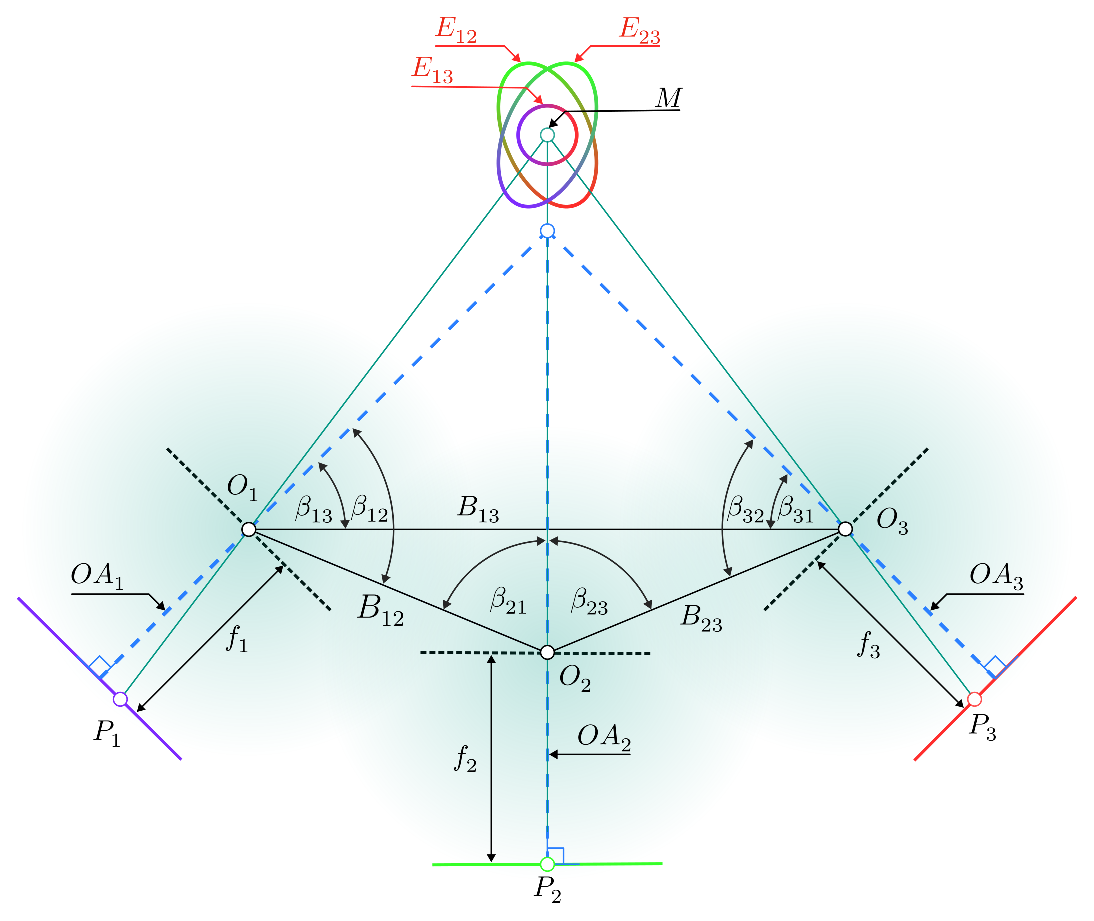
\includegraphics[width=0.8\linewidth]{graphics/MixedErrorCuttingGeometry.eps}
	\caption{Top view of a photogrammetric sensor in trifocal configuration under simplified converging geometric constraints, wherby the optical axes $OA$ of three cameras systems intersect in one point $\mathbf{I}$.		
	It can also be regarded as the composition of $n_{sub}=3$ stereoscopic subsystems, whereby the measurement error of each subsystem corresponds in shape to an ellipsoid $\mathbf{E}$.}
	\label{fig:sub_sensors}
\end{figure}

\subsection{Optimized Perception}
It has been remarked in the literature~\cite{Di_Leo_2011} that a covariance exists between the input quantities of a stereoscopic system and it is related to a combination of marker and the image processing algorithm used for detection.
Only recently, for the case of a simplified stereoscopic sensor under converging constraints with passive markers, simulation results have experimentally been verified.
Liu et al.~\cite{Liu_2021} showed that the optimum camera orientation angle $\beta_{mn}$ is in the scope of $60^{\circ} --\, 80^{\circ}$, not $30^{\circ} \text{-}\, 50^{\circ}$ \cite{Yang2018,Fooladgar2013,Sankowski2017}.

The input quantities for such a system are depicted in Fig.~\ref{fig:sub_sensors} and read
\begin{equation*}
	\mathbf{Q}= \left[x’_m, y’_m, x’_n, y’_n, \beta_{mn}, \beta_{nm}, B_{nm}, f_{n},f_{m}\right]^{\top}
\end{equation*}
In this case $x’, y’$ is the pixel position of the marker on the sensor plane, $\beta$ is the aforementioned camera orientation angle, $B$ is the distance between the pinhole position and $f$ is the focal length. \\
 
The covariance matrix becomes
\begin{equation}
	\label{eqn:CovarianceMatrix}
	\mathbf{\Lambda_{Q}} = 
	\begin{bmatrix}
		\sigma_{\delta_1}^2  & 0 & 0 & 0 & \sigma_{(\delta_1,\delta_5)}^2 & 0 & 0 & 0 & 0 \\
		0  & \sigma_{\delta_2}^2 & 0 & 0 & \sigma_{(\delta_2,\delta_5)}^2 & 0 & 0 & 0 & 0 \\
		0 & 0 & \sigma_{\delta_3}^2 & 0 & 0 & \sigma_{(\delta_3,\delta_6)}^2 & 0 & 0 & 0 \\
		0 & 0 & 0 & \sigma_{\delta_4}^2 & 0 & \sigma_{(\delta_4,\delta_6)}^2 & 0 & 0 & 0 \\
		\sigma_{(\delta_5,\delta_1)}^2 & \sigma_{(\delta_5,\delta_2)}^2 & 0 & 0 & \sigma_{\delta_5}^2 & 0 & 0 & 0 & 0 \\
		0 & 0 & \sigma_{(\delta_6,\delta_3)}^2 & \sigma_{(\delta_6,\delta_4)}^2 & 0 & \sigma_{\delta_6}^2 & 0 & 0 & 0 \\
		0 & 0 & 0 & 0 & 0 & 0 & \sigma_{\delta_7}^2 & 0 & 0 \\
		0 & 0 & 0 & 0 & 0 & 0 & 0 & \sigma_{\delta_8}^2 & 0 \\
		0 & 0 & 0 & 0 & 0 & 0 & 0 & 0 & \sigma_{\delta_9}^2
	\end{bmatrix}
\end{equation}
Therein, the off-diagonal elements represent the cross-correlation between the camera orientation angle $\beta$ and the point position $x,y$ on the detector.
This correlation is related to the decreasing visible surface of the passive markers, which leads to an increase of the effective noise per area.\\

\begin{figure}[!htb]
	\centering
	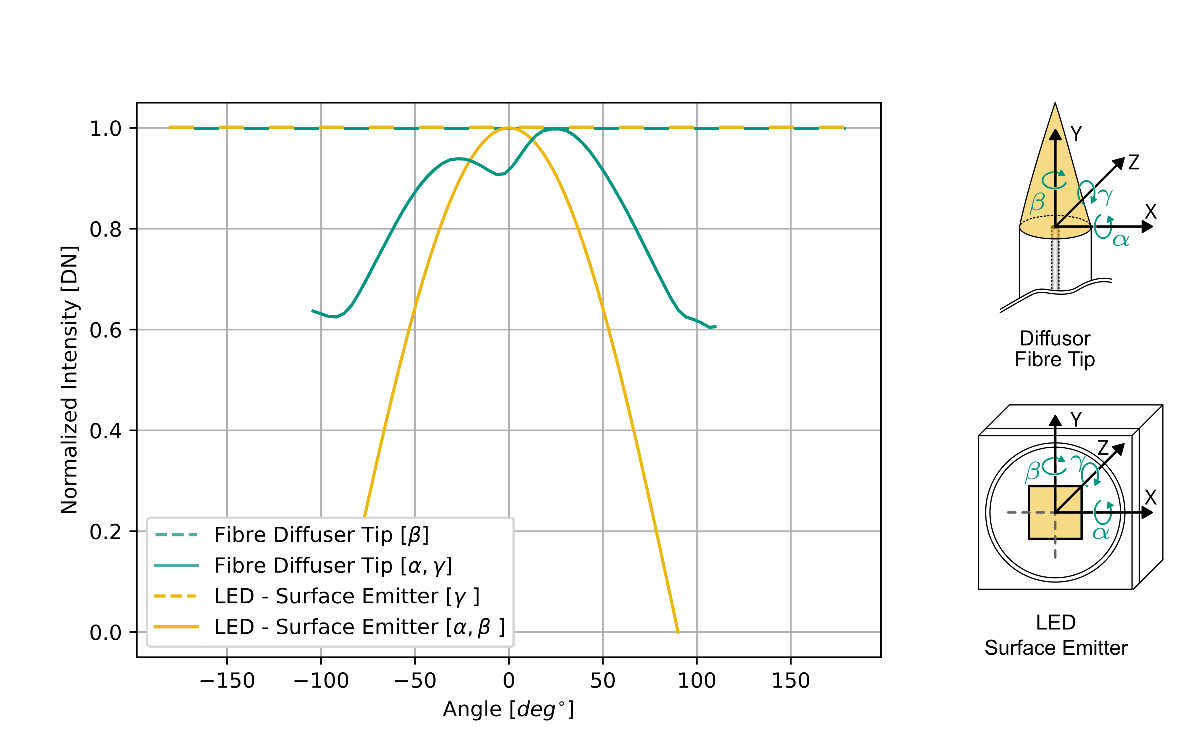
\includegraphics[width=0.95\linewidth]{graphics/ScatteringProfile_DiffuseFibreTip.eps}
	\caption{Radiation characteristic of an LED and diffusor fiber tip and the corresponding frame of reference.}
	\label{fig:scat_profile}
\end{figure}

Since multipoint detection \cite{Haist2015} uses sub-resolution active markers instead of passive ones, it cannot be assumed that the cross-correlation factors are similar. Since here the so called signal-to-noise Ratio (SNR) primarily depends on intensity of the spots on the sensor plane. \\
This signal strength is on the one hand related to the distance between sensor and marker \cite{dumbleton1955}, on the other hand it depends on the spatial orientation of the marker in regards to the receiving optic. As depicted in Fig.~\ref{fig:scat_profile}
the radiation characteristic of a LED or a diffusor fiber tip \cite{Pan1994} is for most angular orientations non-isotropic.\\

\begin{figure}[!htb]
	\centering
	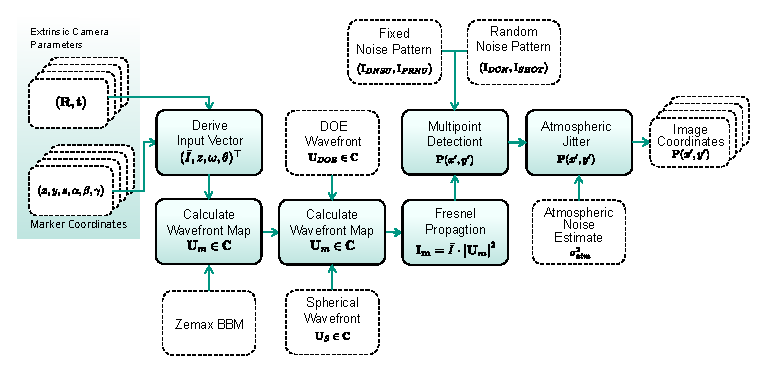
\includegraphics[width=\columnwidth]{graphics/OpticalSimulation.eps}
	\caption{Simulation procedure for multipoint detection based on a Zemax Black-Box-Model (BBM) and a combination of geometric and Fresnel propagation.}
	\label{fig:opto-sim}
\end{figure}

On this basis an optical simulation procedure was created, as can be seen in Fig.~\ref{fig:opto-sim}, to extended previous works \cite{Liu_2021,Di_Leo_2011} about the covariance-analysis for stereoscopic sensors.
\\
In this case the extrinsic camera parameters and the marker coordinates in space and orientation are used to derive
the input vector for the simulation, which comprises information about the normalized intensity distribution $\bar{I}$, the distance to marker $z$ and the field angles $\omega$ and $\theta$. A Zemax Black Box Model of the lens is used to compute the complex wavefront distribution at the DOE-Position $\mathbf{U}_m$, which is combined with the DOE Phase Distribution and $\mathbf{U}_{DOE}$ a spherical Wavefront $\mathbf{U}_{S}$ to accommodate for the distance of the DOE to the imager. This Wavefront is propagated onto the sensor by the Fresnel method \cite{Goodman2005}. The fixed $\mathbf{I}_{DNSU/PRNU}$ and random $\mathbf{I}_{DCN/SHOT}$ noise patterns are superimposed onto the derived sensor intensity distribution $\mathbf{I}_m$ and the point coordinates $P_{x’,y’}$ are derived via multipoint detection.
Finally the point position is varied by an estimate of the atmospheric disturbance.\\


\textbf{
If the robot end effector is obscured and the optical measurement system cannot detect its pose (position and orientation), the pose of the endeffector is estimated using a Kalman filter with a constant velocity model. This assumption is reasonable in this case, as the measurement rate of the measurement system is significantly higher than the change in the pose of the endeffector.}

\textbf{
je mehr Kameras, desto besser die Aufloesung \\
- natuerlicherweise sos \\
- man braucht Strategie diese zu platzieren, siehe process strategies, camera placement \\
so platzieren, dass sie das Target ueberhaupt sehen, nur damit bringen mehr Kameras auch Verbesserung }

% 
Intuitively, one would state that more cameras lead to a smaller metrological error
\textcolor{red}{Referenz auf welche Formel?}
The restriction, however is, that they need to be placed such that they can perceive the target at all -- only then more cameras lead to an improved perception.
Therefore, a strategy to place the cameras is presented as a part of the process strategies in the next section.

\section{Process Strategies}
\subsection{Hardware implementation} 

Kameras, Setup beschreiben (mehr als 2 Kameras wg. Abschattung, ergibt sich aus zuvor beschriebener Theorie)


of control system: robot w/ external sensor
calibration of camera system: interface ITO / ISYS
synchronized measurements of the camera, joint angles (encoders), joint torques 
interface through which the reference values for the joint space position, velocity and acceleration are directly communicated to the built-in robot trajectory tracking controller

pneumatic robot - direct drives, drive dynamics 

\subsection{overall strategy in software}
To find a compromise between accuracy and speed, the motion planning problem is divided into path planning and path trajectory generation, which is a common approach in the literature~\cite{Choset05}.
In path planning, the path of each of the robot’s joint angles is computed, providing the highest possible repeatability.
In trajectory generation, the previously computed path is indexed in time so that the robot can follow the given paths as quickly as possible such that the process speed is maximized, taking into account dynamic constraints of the robot (e.g. actuator dynamics).
\\
% Kinematic and dynamic strategies need to be separated. 
% In the field of robot trajectory generation, this has lead to the path speed decomposition framework~\cite{Choset05}, which is well known in the literature. 
% Therein, first a path is generated kinematically, and second time-indexed considering the robot dynamics. 
This also allows for a separate consideration of kinematic and dynamic errors of the robot system. 

\subsection{Kinematic strategies:}
Some kinematic strategies for increasing the accuracy of industrial robots are already well-established.
Purely geometric errors in a robot can stem from the sources length deviations of links, axis misalignment and zero-position offsets of the encoders.
There are established methods for identifying and compensating these parameters in an offline calibration technique~\cite{Wiest01}.
To this end, the endeffector pose is measured with an external measurement statically at certain points in the workspace and a certain number of times, and the geometric error parameters are determined in an optimization.
This offline calibration is usually performed at certain points, because of which it does not generalize in the entire workspace and is not applicable in the industrial robot application itself, but provides a first enhanced kinematic model of the robot.
From a kinematic point of view, if the manufacturing tolerances of the robot are known, incorporating them in the forward kinematics yields an error measure in task space. Such errors are usually much larger than the measurement accuracy of the presented measurement system.

It also captures the static deformation of the robot structure, which cannot be sep
different under different loads 

\subsection{Path Planning}
There are several error sources impeding the accuracy of a robotic manufacturing system.
An overview of these sources can be seen in Fig.~\ref{fig:error_sources}.
Most of these errors can be captured with the present measurement system and from that be compensated.

This leaves the finite precision of the robot itself, whose contribution can not be compensated but only mitigated.
Previous works such as \cite{previous_work} have shown that the optimal repeatability of a path is dependent on the workpiece placement.
This means that we can use the workpiece holding robot to reposition the workpiece in such a way that the optimal repeatability is achieved.
It might be tempting to try to find a continuous trajectory of this second robot to minimize the error.
However the second robot also suffers under finite joint precision, while moving these will introduce additional errors.
It is therefore better if the workpiece holding robot moves to a fixed position before the second robot starts moving.
This leads to a two step process similar to the one described in \cite{stroke_division}.
Here the authors propose a 4 step process to path planning:
\begin{enumerate}
	\item Cut path into multiple segments
	\item Downsample each segment
	\item Optimize the pose of each subpath and compute the joint path
	\item Apply the new pose to the original segments
\end{enumerate}
The division of the path into multiple segments was performed by identifying turning points using path simplification algorithms \cite{stroke_division}.
However instead of using the pose optimization algorithm described in \cite{stroke_division} we use the problem formulation of \cite{previous_work} since it allows us to integrate more constraints which are later used for the joint trajectory optimization.
% Hier ein Experiment durchführen mit den FESTO Robotern und zeigen wie sich die Genauigkeit gegen die Anzahl der Segmente verhält.
% Hier kann man dann als nächstes die Genauigkeit gegen die Taktzeit auftragen wenn man die Anzahl der Segmente variiert. Hier wird sich Pareto Kurve ergeben.


% The optimal Repeatability is dependent on the optimized kinematic parameters.




\subsection{Dynamic Strategies:} Ongoing Research \\
literature on capturing dynamic errors:

here: present robot’s drives are direct drives, therefore no backlash in gearing, joint angle tracking error directly measured, 
enables dynamic error model
alternative: secondary encoders~\cite{Mesmer22}

closed loop control of the robot joints: tracking errors occur, but are captured in joint angle measurement

dynamic error model

data from measurement: same path executed at different speeds - dynamic error model is able to predict dynamic error of other velocity profile,

\begin{figure}[h]
	\centering
	% This file was created by matlab2tikz.
%
\definecolor{mycolor1}{HTML}{009682}%
\definecolor{mycolor2}{HTML}{eeb70d}%
%\definecolor{mycolor3}{rgb}{0.00000,0.44700,0.74100}%
%
\begin{tikzpicture}[%
scale=1.0
]

\begin{axis}[%
width=7cm,
height=3cm,
at={(0cm,0cm)},
scale only axis,
xmin=0,
xmax=6.44,
xlabel style={font=\color{white!15!black},font=\small},
xlabel={$t$ in s},
ymin=-1.4241,
ymax=1.5759,
ylabel style={font=\color{white!15!black},font=\small},
ylabel={$e$ in deg},
%ylabel shift=-2pt,
axis background/.style={fill=white},
xmajorgrids,
ymajorgrids,
legend style={at={(0.05,0.7)}, anchor=south west, legend cell align=left, align=left, draw=white!15!black, font=\small, inner sep=0pt}
]
\addplot [color=mycolor1, line width=1pt]
  table[row sep=crcr]{%
0.01	0.17011\\
0.02	0.12017\\
0.03	0.042693\\
0.04	-0.026964\\
0.05	-0.11627\\
0.06	-0.17846\\
0.07	-0.23972\\
0.08	-0.31375\\
0.09	-0.38496\\
0.1	-0.4316\\
0.11	-0.47015\\
0.12	-0.51056\\
0.13	-0.52567\\
0.14	-0.52196\\
0.15	-0.50266\\
0.16	-0.47305\\
0.17	-0.44826\\
0.18	-0.41772\\
0.19	-0.39181\\
0.2	-0.37056\\
0.21	-0.33645\\
0.22	-0.30374\\
0.23	-0.2602\\
0.24	-0.22747\\
0.25	-0.19703\\
0.26	-0.17555\\
0.27	-0.14818\\
0.28	-0.11683\\
0.29	-0.10184\\
0.3	-0.076948\\
0.31	-0.043035\\
0.32	-0.0054098\\
0.33	0.028987\\
0.34	0.067121\\
0.35	0.099356\\
0.36	0.12457\\
0.37	0.14397\\
0.38	0.15883\\
0.39	0.17323\\
0.4	0.18081\\
0.41	0.18756\\
0.42	0.18804\\
0.43	0.19223\\
0.44	0.19669\\
0.45	0.19982\\
0.46	0.21275\\
0.47	0.22831\\
0.48	0.24546\\
0.49	0.26009\\
0.5	0.27127\\
0.51	0.27823\\
0.52	0.27751\\
0.53	0.26402\\
0.54	0.24924\\
0.55	0.22424\\
0.56	0.19817\\
0.57	0.17602\\
0.58	0.14675\\
0.59	0.11898\\
0.6	0.094032\\
0.61	0.071498\\
0.62	0.044427\\
0.63	0.023269\\
0.64	0.0048316\\
0.65	-0.007004\\
0.66	-0.016546\\
0.67	-0.026752\\
0.68	-0.037031\\
0.69	-0.036459\\
0.7	-0.035067\\
0.71	-0.032255\\
0.72	-0.030207\\
0.73	-0.024747\\
0.74	-0.018278\\
0.75	-0.014259\\
0.76	-0.011251\\
0.77	-0.010811\\
0.78	-0.012282\\
0.79	-0.020049\\
0.8	-0.03411\\
0.81	-0.050989\\
0.82	-0.068897\\
0.83	-0.094926\\
0.84	-0.12103\\
0.85	-0.14528\\
0.86	-0.16399\\
0.87	-0.17939\\
0.88	-0.1891\\
0.89	-0.1883\\
0.9	-0.18318\\
0.91	-0.17009\\
0.92	-0.14696\\
0.93	-0.12581\\
0.94	-0.096685\\
0.95	-0.063796\\
0.96	-0.031632\\
0.97	0.00087785\\
0.98	0.030169\\
0.99	0.057312\\
1	0.073107\\
1.01	0.088355\\
1.02	0.098519\\
1.03	0.10594\\
1.04	0.11215\\
1.05	0.11535\\
1.06	0.11916\\
1.07	0.12464\\
1.08	0.12931\\
1.09	0.12804\\
1.1	0.12181\\
1.11	0.11959\\
1.12	0.11995\\
1.13	0.11459\\
1.14	0.10848\\
1.15	0.10219\\
1.16	0.10785\\
1.17	0.10234\\
1.18	0.091444\\
1.19	0.065481\\
1.2	0.045761\\
1.21	0.011353\\
1.22	-0.029841\\
1.23	-0.082939\\
1.24	-0.12963\\
1.25	-0.16235\\
1.26	-0.19835\\
1.27	-0.23416\\
1.28	-0.24306\\
1.29	-0.23558\\
1.3	-0.22897\\
1.31	-0.19332\\
1.32	-0.15511\\
1.33	-0.10783\\
1.34	-0.053153\\
1.35	0.0050455\\
1.36	0.059025\\
1.37	0.10385\\
1.38	0.13147\\
1.39	0.14987\\
1.4	0.15727\\
1.41	0.15249\\
1.42	0.13234\\
1.43	0.11651\\
1.44	0.094064\\
1.45	0.089954\\
1.46	0.080845\\
1.47	0.08658\\
1.48	0.05931\\
1.49	0.034732\\
1.5	-0.011556\\
1.51	-0.029858\\
1.52	-0.076545\\
1.53	-0.1155\\
1.54	-0.15854\\
1.55	-0.17905\\
1.56	-0.20568\\
1.57	-0.23162\\
1.58	-0.26545\\
1.59	-0.2913\\
1.6	-0.31644\\
1.61	-0.32186\\
1.62	-0.32312\\
1.63	-0.29164\\
1.64	-0.27551\\
1.65	-0.24588\\
1.66	-0.22656\\
1.67	-0.20099\\
1.68	-0.18856\\
1.69	-0.18207\\
1.7	-0.18128\\
1.71	-0.17923\\
1.72	-0.18793\\
1.73	-0.17782\\
1.74	-0.16871\\
1.75	-0.13799\\
1.76	-0.10396\\
1.77	-0.07032\\
1.78	-0.031301\\
1.79	0.0075125\\
1.8	0.034597\\
1.81	0.054354\\
1.82	0.073733\\
1.83	0.08338\\
1.84	0.08768\\
1.85	0.094028\\
1.86	0.096082\\
1.87	0.09648\\
1.88	0.098416\\
1.89	0.097968\\
1.9	0.093238\\
1.91	0.089883\\
1.92	0.089135\\
1.93	0.078941\\
1.94	0.073321\\
1.95	0.064314\\
1.96	0.043542\\
1.97	0.021013\\
1.98	-0.0017352\\
1.99	-0.031666\\
2	-0.060316\\
2.01	-0.0798\\
2.02	-0.10557\\
2.03	-0.11936\\
2.04	-0.13828\\
2.05	-0.14998\\
2.06	-0.17111\\
2.07	-0.18726\\
2.08	-0.18657\\
2.09	-0.19785\\
2.1	-0.20649\\
2.11	-0.21451\\
2.12	-0.21617\\
2.13	-0.21913\\
2.14	-0.22517\\
2.15	-0.20535\\
2.16	-0.19119\\
2.17	-0.1489\\
2.18	-0.1135\\
2.19	-0.06341\\
2.2	-0.020291\\
2.21	0.0027406\\
2.22	0.029641\\
2.23	0.045225\\
2.24	0.063457\\
2.25	0.087074\\
2.26	0.11171\\
2.27	0.14177\\
2.28	0.19002\\
2.29	0.2473\\
2.3	0.27724\\
2.31	0.30774\\
2.32	0.32602\\
2.33	0.33288\\
2.34	0.33252\\
2.35	0.33878\\
2.36	0.34071\\
2.37	0.33576\\
2.38	0.33121\\
2.39	0.32374\\
2.4	0.32213\\
2.41	0.31202\\
2.42	0.31133\\
2.43	0.31344\\
2.44	0.3164\\
2.45	0.31132\\
2.46	0.29646\\
2.47	0.26211\\
2.48	0.20039\\
2.49	0.13803\\
2.5	0.050147\\
2.51	-0.023404\\
2.52	-0.094143\\
2.53	-0.1332\\
2.54	-0.16767\\
2.55	-0.17943\\
2.56	-0.16884\\
2.57	-0.15538\\
2.58	-0.13163\\
2.59	-0.094477\\
2.6	-0.076383\\
2.61	-0.051008\\
2.62	-0.024549\\
2.63	-0.0045232\\
2.64	0.010228\\
2.65	0.017809\\
2.66	0.02054\\
2.67	0.018399\\
2.68	0.012204\\
2.69	0.0059981\\
2.7	-0.00017694\\
2.71	-0.006703\\
2.72	-0.016228\\
2.73	-0.027662\\
2.74	-0.043237\\
2.75	-0.066079\\
2.76	-0.09492\\
2.77	-0.12869\\
2.78	-0.17454\\
2.79	-0.20658\\
2.8	-0.24959\\
2.81	-0.29021\\
2.82	-0.32572\\
2.83	-0.34033\\
2.84	-0.32701\\
2.85	-0.33215\\
2.86	-0.32651\\
2.87	-0.3004\\
2.88	-0.2768\\
2.89	-0.28247\\
2.9	-0.28168\\
2.91	-0.28527\\
2.92	-0.30549\\
2.93	-0.32597\\
2.94	-0.34009\\
2.95	-0.35583\\
2.96	-0.35933\\
2.97	-0.3707\\
2.98	-0.36692\\
2.99	-0.34939\\
3	-0.33205\\
3.01	-0.29605\\
3.02	-0.23831\\
3.03	-0.18694\\
3.04	-0.10082\\
3.05	-0.029947\\
3.06	0.033312\\
3.07	0.084064\\
3.08	0.1183\\
3.09	0.13237\\
3.1	0.13355\\
3.11	0.12122\\
3.12	0.11465\\
3.13	0.11831\\
3.14	0.12211\\
3.15	0.13282\\
3.16	0.12116\\
3.17	0.14634\\
3.18	0.15167\\
3.19	0.12724\\
3.2	0.11967\\
3.21	0.11436\\
3.22	0.12606\\
3.23	0.13621\\
3.24	0.14108\\
3.25	0.15536\\
3.26	0.18896\\
3.27	0.22632\\
3.28	0.25784\\
3.29	0.29798\\
3.3	0.33141\\
3.31	0.35904\\
3.32	0.36732\\
3.33	0.37599\\
3.34	0.37739\\
3.35	0.38368\\
3.36	0.39055\\
3.37	0.41137\\
3.38	0.42161\\
3.39	0.41992\\
3.4	0.41644\\
3.41	0.40787\\
3.42	0.39032\\
3.43	0.38114\\
3.44	0.37028\\
3.45	0.35796\\
3.46	0.3454\\
3.47	0.33259\\
3.48	0.32809\\
3.49	0.32194\\
3.5	0.31372\\
3.51	0.31428\\
3.52	0.31415\\
3.53	0.31408\\
3.54	0.30257\\
3.55	0.27301\\
3.56	0.22567\\
3.57	0.15363\\
3.58	0.073002\\
3.59	-0.0037207\\
3.6	-0.087987\\
3.61	-0.14646\\
3.62	-0.16119\\
3.63	-0.16224\\
3.64	-0.12823\\
3.65	-0.073517\\
3.66	-0.041009\\
3.67	-0.012671\\
3.68	0.0047235\\
3.69	0.013327\\
3.7	0.019693\\
3.71	0.030284\\
3.72	0.045386\\
3.73	0.059944\\
3.74	0.070575\\
3.75	0.076643\\
3.76	0.078713\\
3.77	0.076159\\
3.78	0.067689\\
3.79	0.057183\\
3.8	0.038454\\
3.81	0.0095434\\
3.82	-0.023994\\
3.83	-0.070896\\
3.84	-0.12614\\
3.85	-0.18401\\
3.86	-0.24044\\
3.87	-0.28979\\
3.88	-0.32529\\
3.89	-0.35849\\
3.9	-0.37954\\
3.91	-0.37976\\
3.92	-0.38184\\
3.93	-0.38434\\
3.94	-0.3795\\
3.95	-0.34286\\
3.96	-0.34915\\
3.97	-0.31513\\
3.98	-0.30292\\
3.99	-0.31857\\
4	-0.3653\\
4.01	-0.41978\\
4.02	-0.43494\\
4.03	-0.45778\\
4.04	-0.49319\\
4.05	-0.48171\\
4.06	-0.4814\\
4.07	-0.49663\\
4.08	-0.50878\\
4.09	-0.47899\\
4.1	-0.46492\\
4.11	-0.44643\\
4.12	-0.34456\\
4.13	-0.25452\\
4.14	-0.1676\\
4.15	-0.063741\\
4.16	0.02275\\
4.17	0.079898\\
4.18	0.11882\\
4.19	0.11464\\
4.2	0.10059\\
4.21	0.086879\\
4.22	0.07484\\
4.23	0.063328\\
4.24	0.10357\\
4.25	0.14327\\
4.26	0.12783\\
4.27	0.080852\\
4.28	0.048706\\
4.29	0.0050957\\
4.3	-0.068042\\
4.31	-0.12075\\
4.32	-0.1535\\
4.33	-0.1863\\
4.34	-0.21474\\
4.35	-0.24688\\
4.36	-0.2513\\
4.37	-0.2748\\
4.38	-0.27815\\
4.39	-0.27198\\
4.4	-0.27231\\
4.41	-0.2528\\
4.42	-0.21515\\
4.43	-0.17855\\
4.44	-0.14336\\
4.45	-0.092759\\
4.46	-0.039329\\
4.47	-0.0031933\\
4.48	0.027311\\
4.49	0.06108\\
4.5	0.080729\\
4.51	0.10368\\
4.52	0.14169\\
4.53	0.18651\\
4.54	0.21809\\
4.55	0.24437\\
4.56	0.25967\\
4.57	0.25307\\
4.58	0.22722\\
4.59	0.19229\\
4.6	0.16084\\
4.61	0.14311\\
4.62	0.12478\\
4.63	0.12036\\
4.64	0.13992\\
4.65	0.1561\\
4.66	0.17377\\
4.67	0.19118\\
4.68	0.20445\\
4.69	0.21106\\
4.7	0.22442\\
4.71	0.23653\\
4.72	0.25376\\
4.73	0.27046\\
4.74	0.27364\\
4.75	0.26853\\
4.76	0.23298\\
4.77	0.17174\\
4.78	0.089602\\
4.79	-0.014567\\
4.8	-0.11042\\
4.81	-0.2056\\
4.82	-0.26993\\
4.83	-0.28274\\
4.84	-0.23638\\
4.85	-0.13268\\
4.86	-0.026872\\
4.87	0.052786\\
4.88	0.057446\\
4.89	-0.047835\\
4.9	-0.25593\\
4.91	-0.42726\\
4.92	-0.65618\\
4.93	-0.77891\\
4.94	-0.89434\\
4.95	-0.96445\\
4.96	-0.96735\\
4.97	-0.91849\\
4.98	-0.84636\\
4.99	-0.71512\\
5	-0.57473\\
5.01	-0.41833\\
5.02	-0.27818\\
5.03	-0.1603\\
5.04	-0.068829\\
5.05	0.0066623\\
5.06	0.071331\\
5.07	0.11661\\
5.08	0.1881\\
5.09	0.29063\\
5.1	0.39681\\
5.11	0.51732\\
5.12	0.60128\\
5.13	0.66533\\
5.14	0.67841\\
5.15	0.64226\\
5.16	0.56296\\
5.17	0.47836\\
5.18	0.37049\\
5.19	0.29961\\
5.2	0.25043\\
5.21	0.22573\\
5.22	0.21304\\
5.23	0.1917\\
5.24	0.14699\\
5.25	0.084434\\
5.26	0.034966\\
5.27	-0.0045612\\
5.28	0.00040138\\
5.29	0.015943\\
5.3	0.039735\\
5.31	0.048972\\
5.32	0.034297\\
5.33	0.013474\\
5.34	-0.0016241\\
5.35	-0.0014831\\
5.36	0.018153\\
5.37	0.046258\\
5.38	0.073686\\
5.39	0.097452\\
5.4	0.10466\\
5.41	0.102\\
5.42	0.094969\\
5.43	0.085849\\
5.44	0.078093\\
5.45	0.079022\\
5.46	0.096449\\
5.47	0.10714\\
5.48	0.12284\\
5.49	0.16039\\
5.5	0.21247\\
5.51	0.21045\\
5.52	0.25656\\
5.53	0.29848\\
5.54	0.37047\\
5.55	0.41938\\
5.56	0.44568\\
5.57	0.50886\\
5.58	0.5385\\
5.59	0.55895\\
5.6	0.51983\\
5.61	0.59319\\
5.62	0.61052\\
5.63	0.56733\\
5.64	0.54592\\
5.65	0.56271\\
5.66	0.46084\\
5.67	0.4087\\
5.68	0.41321\\
5.69	0.33298\\
5.7	0.17901\\
5.71	0.12091\\
5.72	0.021071\\
5.73	-0.07222\\
5.74	-0.037428\\
5.75	-0.050942\\
5.76	0.038752\\
5.77	0.11169\\
5.78	0.20134\\
5.79	0.23935\\
5.8	0.23498\\
5.81	0.2154\\
5.82	0.20303\\
5.83	0.16583\\
5.84	0.20194\\
5.85	0.19389\\
5.86	0.1901\\
5.87	0.24469\\
5.88	0.22834\\
5.89	0.13336\\
5.9	0.11202\\
5.91	0.068427\\
5.92	0.018356\\
5.93	-0.033536\\
5.94	-0.090402\\
5.95	-0.17482\\
5.96	-0.2632\\
5.97	-0.34631\\
5.98	-0.41766\\
5.99	-0.49266\\
6	-0.57878\\
6.01	-0.68405\\
6.02	-0.77374\\
6.03	-0.86611\\
6.04	-0.95115\\
6.05	-1.005\\
6.06	-1.0544\\
6.07	-1.0717\\
6.08	-1.0846\\
6.09	-1.0939\\
6.1	-1.0858\\
6.11	-1.1064\\
6.12	-1.1246\\
6.13	-1.1275\\
6.14	-1.1504\\
6.15	-1.1681\\
6.16	-1.175\\
6.17	-1.1802\\
6.18	-1.1681\\
6.19	-1.1013\\
6.2	-1.038\\
6.21	-0.98208\\
6.22	-0.91998\\
6.23	-0.84766\\
6.24	-0.80769\\
6.25	-0.73338\\
6.26	-0.6736\\
6.27	-0.59834\\
6.28	-0.49431\\
6.29	-0.40241\\
6.3	-0.30379\\
6.31	-0.2473\\
6.32	-0.1841\\
6.33	-0.12768\\
6.34	-0.079534\\
6.35	-0.050641\\
6.36	0.031593\\
6.37	0.096518\\
6.38	0.1596\\
6.39	0.22969\\
6.4	0.28045\\
6.41	0.32269\\
6.42	0.3598\\
6.43	0.35625\\
6.44	0.33653\\
};
\addlegendentry{GP}
%
\addplot [color=mycolor2, line width=1pt]
  table[row sep=crcr]{%
0.01	-0.13159\\
0.02	-0.14921\\
0.03	-0.1658\\
0.04	-0.1803\\
0.05	-0.19292\\
0.06	-0.21406\\
0.07	-0.23164\\
0.08	-0.23994\\
0.09	-0.24682\\
0.1	-0.25897\\
0.11	-0.2689\\
0.12	-0.27135\\
0.13	-0.26763\\
0.14	-0.27261\\
0.15	-0.26882\\
0.16	-0.2554\\
0.17	-0.24378\\
0.18	-0.23148\\
0.19	-0.2122\\
0.2	-0.18933\\
0.21	-0.1564\\
0.22	-0.12905\\
0.23	-0.095083\\
0.24	-0.072844\\
0.25	-0.042728\\
0.26	-0.010431\\
0.27	0.027194\\
0.28	0.060234\\
0.29	0.079679\\
0.3	0.097084\\
0.31	0.11461\\
0.32	0.12371\\
0.33	0.15264\\
0.34	0.17388\\
0.35	0.19123\\
0.36	0.20388\\
0.37	0.2043\\
0.38	0.21368\\
0.39	0.21541\\
0.4	0.21029\\
0.41	0.20749\\
0.42	0.20623\\
0.43	0.19775\\
0.44	0.1887\\
0.45	0.18012\\
0.46	0.18249\\
0.47	0.18332\\
0.48	0.18533\\
0.49	0.18733\\
0.5	0.18657\\
0.51	0.18721\\
0.52	0.18715\\
0.53	0.18575\\
0.54	0.18157\\
0.55	0.1732\\
0.56	0.16621\\
0.57	0.15514\\
0.58	0.14403\\
0.59	0.12893\\
0.6	0.11869\\
0.61	0.11094\\
0.62	0.099089\\
0.63	0.096041\\
0.64	0.098957\\
0.65	0.10143\\
0.66	0.10384\\
0.67	0.10118\\
0.68	0.098778\\
0.69	0.093989\\
0.7	0.08729\\
0.71	0.077748\\
0.72	0.067668\\
0.73	0.049953\\
0.74	0.031897\\
0.75	0.010916\\
0.76	-6.1472e-05\\
0.77	-0.015682\\
0.78	-0.035273\\
0.79	-0.055888\\
0.8	-0.083421\\
0.81	-0.11105\\
0.82	-0.13905\\
0.83	-0.17202\\
0.84	-0.20187\\
0.85	-0.22318\\
0.86	-0.22894\\
0.87	-0.22564\\
0.88	-0.22604\\
0.89	-0.22379\\
0.9	-0.22596\\
0.91	-0.22525\\
0.92	-0.20212\\
0.93	-0.1825\\
0.94	-0.16566\\
0.95	-0.1524\\
0.96	-0.13576\\
0.97	-0.11391\\
0.98	-0.093715\\
0.99	-0.071398\\
1	-0.05584\\
1.01	-0.044938\\
1.02	-0.032298\\
1.03	-0.018486\\
1.04	-0.0041801\\
1.05	0.0011663\\
1.06	-0.0031829\\
1.07	-0.00045079\\
1.08	0.0068404\\
1.09	0.014719\\
1.1	0.0046565\\
1.11	-0.010887\\
1.12	-0.021484\\
1.13	-0.026513\\
1.14	-0.027946\\
1.15	-0.027968\\
1.16	-0.041203\\
1.17	-0.056542\\
1.18	-0.073025\\
1.19	-0.088181\\
1.2	-0.097206\\
1.21	-0.10406\\
1.22	-0.10854\\
1.23	-0.10981\\
1.24	-0.1065\\
1.25	-0.099178\\
1.26	-0.085721\\
1.27	-0.070732\\
1.28	-0.068565\\
1.29	-0.056795\\
1.3	-0.041922\\
1.31	-0.025465\\
1.32	-0.0028072\\
1.33	0.021834\\
1.34	0.049869\\
1.35	0.080929\\
1.36	0.11144\\
1.37	0.12515\\
1.38	0.13191\\
1.39	0.12561\\
1.4	0.11906\\
1.41	0.11619\\
1.42	0.1183\\
1.43	0.11143\\
1.44	0.08151\\
1.45	0.051571\\
1.46	0.030579\\
1.47	0.0094052\\
1.48	-0.02582\\
1.49	-0.055757\\
1.5	-0.082406\\
1.51	-0.10691\\
1.52	-0.14225\\
1.53	-0.16881\\
1.54	-0.18939\\
1.55	-0.2145\\
1.56	-0.23197\\
1.57	-0.24674\\
1.58	-0.25621\\
1.59	-0.26255\\
1.6	-0.27069\\
1.61	-0.26691\\
1.62	-0.26452\\
1.63	-0.26246\\
1.64	-0.25212\\
1.65	-0.24281\\
1.66	-0.23553\\
1.67	-0.22295\\
1.68	-0.20772\\
1.69	-0.194\\
1.7	-0.18066\\
1.71	-0.16404\\
1.72	-0.15305\\
1.73	-0.13528\\
1.74	-0.1242\\
1.75	-0.10795\\
1.76	-0.092518\\
1.77	-0.080674\\
1.78	-0.069207\\
1.79	-0.050083\\
1.8	-0.038819\\
1.81	-0.02221\\
1.82	-0.0137\\
1.83	-0.00064972\\
1.84	0.0090184\\
1.85	0.011911\\
1.86	0.018322\\
1.87	0.024833\\
1.88	0.030033\\
1.89	0.031658\\
1.9	0.031637\\
1.91	0.033337\\
1.92	0.029983\\
1.93	0.030132\\
1.94	0.031047\\
1.95	0.024631\\
1.96	0.021842\\
1.97	0.009266\\
1.98	-0.00032785\\
1.99	-0.0095887\\
2	-0.021346\\
2.01	-0.031611\\
2.02	-0.038876\\
2.03	-0.052548\\
2.04	-0.066729\\
2.05	-0.077985\\
2.06	-0.084456\\
2.07	-0.092557\\
2.08	-0.10409\\
2.09	-0.1119\\
2.1	-0.1155\\
2.11	-0.11812\\
2.12	-0.11866\\
2.13	-0.11402\\
2.14	-0.11292\\
2.15	-0.098353\\
2.16	-0.085346\\
2.17	-0.073289\\
2.18	-0.061916\\
2.19	-0.033575\\
2.2	-0.0093621\\
2.21	0.0050637\\
2.22	0.022786\\
2.23	0.061586\\
2.24	0.098155\\
2.25	0.12317\\
2.26	0.13548\\
2.27	0.14614\\
2.28	0.18189\\
2.29	0.21872\\
2.3	0.23823\\
2.31	0.24881\\
2.32	0.25247\\
2.33	0.2466\\
2.34	0.24961\\
2.35	0.24756\\
2.36	0.25153\\
2.37	0.25998\\
2.38	0.26351\\
2.39	0.26136\\
2.4	0.25365\\
2.41	0.24045\\
2.42	0.22641\\
2.43	0.19984\\
2.44	0.17096\\
2.45	0.14022\\
2.46	0.10672\\
2.47	0.065161\\
2.48	0.047187\\
2.49	0.028895\\
2.5	0.012556\\
2.51	-0.0051557\\
2.52	-0.024442\\
2.53	-0.05347\\
2.54	-0.069701\\
2.55	-0.077574\\
2.56	-0.060946\\
2.57	-0.056825\\
2.58	-0.057547\\
2.59	-0.064945\\
2.6	-0.042826\\
2.61	-0.021047\\
2.62	-0.013884\\
2.63	-0.0091332\\
2.64	0.0016222\\
2.65	0.013188\\
2.66	0.016099\\
2.67	0.013888\\
2.68	0.011267\\
2.69	0.0015526\\
2.7	-0.0034966\\
2.71	-0.019141\\
2.72	-0.04241\\
2.73	-0.057084\\
2.74	-0.066996\\
2.75	-0.097398\\
2.76	-0.1263\\
2.77	-0.14944\\
2.78	-0.16439\\
2.79	-0.19102\\
2.8	-0.22995\\
2.81	-0.25154\\
2.82	-0.25733\\
2.83	-0.25848\\
2.84	-0.2842\\
2.85	-0.30594\\
2.86	-0.31453\\
2.87	-0.31719\\
2.88	-0.30761\\
2.89	-0.29143\\
2.9	-0.28285\\
2.91	-0.28136\\
2.92	-0.27732\\
2.93	-0.27616\\
2.94	-0.26967\\
2.95	-0.25787\\
2.96	-0.24111\\
2.97	-0.21945\\
2.98	-0.1879\\
2.99	-0.16144\\
3	-0.11962\\
3.01	-0.081033\\
3.02	-0.03914\\
3.03	-0.0015522\\
3.04	0.021662\\
3.05	0.046122\\
3.06	0.069663\\
3.07	0.098029\\
3.08	0.13102\\
3.09	0.16586\\
3.1	0.17677\\
3.11	0.17999\\
3.12	0.18048\\
3.13	0.18686\\
3.14	0.2022\\
3.15	0.19953\\
3.16	0.18695\\
3.17	0.18302\\
3.18	0.18987\\
3.19	0.18025\\
3.2	0.17149\\
3.21	0.17112\\
3.22	0.17507\\
3.23	0.17832\\
3.24	0.1835\\
3.25	0.18853\\
3.26	0.21067\\
3.27	0.23042\\
3.28	0.24348\\
3.29	0.26041\\
3.3	0.29127\\
3.31	0.3235\\
3.32	0.3426\\
3.33	0.34604\\
3.34	0.38557\\
3.35	0.41607\\
3.36	0.43718\\
3.37	0.44279\\
3.38	0.43592\\
3.39	0.44239\\
3.4	0.44406\\
3.41	0.45851\\
3.42	0.46192\\
3.43	0.46235\\
3.44	0.45596\\
3.45	0.44464\\
3.46	0.43355\\
3.47	0.4132\\
3.48	0.3896\\
3.49	0.36295\\
3.5	0.3293\\
3.51	0.31644\\
3.52	0.29691\\
3.53	0.2721\\
3.54	0.24967\\
3.55	0.2159\\
3.56	0.17966\\
3.57	0.13304\\
3.58	0.085938\\
3.59	0.039153\\
3.6	-0.00053788\\
3.61	-0.031311\\
3.62	-0.035531\\
3.63	-0.047898\\
3.64	-0.06679\\
3.65	-0.096891\\
3.66	-0.098575\\
3.67	-0.075539\\
3.68	-0.067772\\
3.69	-0.076938\\
3.7	-0.067073\\
3.71	-0.038784\\
3.72	-0.025378\\
3.73	-0.029199\\
3.74	-0.011368\\
3.75	-0.0004064\\
3.76	-0.0010621\\
3.77	-0.0053207\\
3.78	-0.009114\\
3.79	-0.015563\\
3.8	-0.027577\\
3.81	-0.054953\\
3.82	-0.075135\\
3.83	-0.08752\\
3.84	-0.12368\\
3.85	-0.17005\\
3.86	-0.19714\\
3.87	-0.21393\\
3.88	-0.24638\\
3.89	-0.30032\\
3.9	-0.32632\\
3.91	-0.33419\\
3.92	-0.33082\\
3.93	-0.36248\\
3.94	-0.3904\\
3.95	-0.40512\\
3.96	-0.40604\\
3.97	-0.39988\\
3.98	-0.38186\\
3.99	-0.37156\\
4	-0.35936\\
4.01	-0.3521\\
4.02	-0.35734\\
4.03	-0.3602\\
4.04	-0.3594\\
4.05	-0.3534\\
4.06	-0.34305\\
4.07	-0.32411\\
4.08	-0.30281\\
4.09	-0.26895\\
4.1	-0.23476\\
4.11	-0.19043\\
4.12	-0.13238\\
4.13	-0.073428\\
4.14	-0.030467\\
4.15	0.00080255\\
4.16	0.037891\\
4.17	0.064718\\
4.18	0.095569\\
4.19	0.13119\\
4.2	0.1766\\
4.21	0.19925\\
4.22	0.19767\\
4.23	0.19674\\
4.24	0.20444\\
4.25	0.2278\\
4.26	0.21011\\
4.27	0.19743\\
4.28	0.1949\\
4.29	0.19862\\
4.3	0.18709\\
4.31	0.1844\\
4.32	0.19322\\
4.33	0.19195\\
4.34	0.20065\\
4.35	0.21249\\
4.36	0.22683\\
4.37	0.24537\\
4.38	0.2682\\
4.39	0.28545\\
4.4	0.31082\\
4.41	0.33309\\
4.42	0.35016\\
4.43	0.37559\\
4.44	0.3977\\
4.45	0.40623\\
4.46	0.416\\
4.47	0.43494\\
4.48	0.44047\\
4.49	0.43728\\
4.5	0.44158\\
4.51	0.45291\\
4.52	0.45554\\
4.53	0.43522\\
4.54	0.42379\\
4.55	0.41159\\
4.56	0.40234\\
4.57	0.39603\\
4.58	0.38077\\
4.59	0.35105\\
4.6	0.33329\\
4.61	0.29806\\
4.62	0.27861\\
4.63	0.25289\\
4.64	0.22558\\
4.65	0.20614\\
4.66	0.17916\\
4.67	0.15373\\
4.68	0.12786\\
4.69	0.10874\\
4.7	0.06628\\
4.71	0.0309\\
4.72	-0.003921\\
4.73	-0.045323\\
4.74	-0.0732\\
4.75	-0.11951\\
4.76	-0.14875\\
4.77	-0.19718\\
4.78	-0.24099\\
4.79	-0.28947\\
4.8	-0.34542\\
4.81	-0.39868\\
4.82	-0.45287\\
4.83	-0.5034\\
4.84	-0.55603\\
4.85	-0.60482\\
4.86	-0.65131\\
4.87	-0.69924\\
4.88	-0.74877\\
4.89	-0.76848\\
4.9	-0.78807\\
4.91	-0.81038\\
4.92	-0.84093\\
4.93	-0.8389\\
4.94	-0.81766\\
4.95	-0.81145\\
4.96	-0.8257\\
4.97	-0.7927\\
4.98	-0.73504\\
4.99	-0.68578\\
5	-0.66314\\
5.01	-0.65021\\
5.02	-0.59814\\
5.03	-0.5191\\
5.04	-0.45456\\
5.05	-0.3995\\
5.06	-0.34848\\
5.07	-0.31763\\
5.08	-0.27952\\
5.09	-0.25809\\
5.1	-0.20321\\
5.11	-0.12344\\
5.12	-0.064964\\
5.13	-0.018264\\
5.14	0.010302\\
5.15	0.015008\\
5.16	0.0034031\\
5.17	-0.022583\\
5.18	-0.056597\\
5.19	-0.09664\\
5.2	-0.14861\\
5.21	-0.20683\\
5.22	-0.25815\\
5.23	-0.27871\\
5.24	-0.27969\\
5.25	-0.26482\\
5.26	-0.21945\\
5.27	-0.1771\\
5.28	-0.12222\\
5.29	-0.074766\\
5.3	-0.029459\\
5.31	0.029963\\
5.32	0.13798\\
5.33	0.26079\\
5.34	0.36083\\
5.35	0.44735\\
5.36	0.57152\\
5.37	0.70192\\
5.38	0.80034\\
5.39	0.89655\\
5.4	1.0125\\
5.41	1.1148\\
5.42	1.2048\\
5.43	1.2672\\
5.44	1.3247\\
5.45	1.3732\\
5.46	1.4308\\
5.47	1.4308\\
5.48	1.4363\\
5.49	1.4604\\
5.5	1.437\\
5.51	1.3848\\
5.52	1.3599\\
5.53	1.3326\\
5.54	1.2765\\
5.55	1.1993\\
5.56	1.1228\\
5.57	1.0763\\
5.58	1.0284\\
5.59	0.9593\\
5.6	0.87134\\
5.61	0.77286\\
5.62	0.70337\\
5.63	0.62557\\
5.64	0.55953\\
5.65	0.50186\\
5.66	0.44032\\
5.67	0.3962\\
5.68	0.36045\\
5.69	0.3454\\
5.7	0.34292\\
5.71	0.33384\\
5.72	0.33987\\
5.73	0.36008\\
5.74	0.38545\\
5.75	0.41476\\
5.76	0.4471\\
5.77	0.47535\\
5.78	0.49938\\
5.79	0.51582\\
5.8	0.48743\\
5.81	0.44366\\
5.82	0.38883\\
5.83	0.348\\
5.84	0.29903\\
5.85	0.22769\\
5.86	0.14336\\
5.87	0.060064\\
5.88	-0.01925\\
5.89	-0.11025\\
5.9	-0.19652\\
5.91	-0.27403\\
5.92	-0.34588\\
5.93	-0.42144\\
5.94	-0.49751\\
5.95	-0.55165\\
5.96	-0.61359\\
5.97	-0.66106\\
5.98	-0.71318\\
5.99	-0.75379\\
6	-0.78682\\
6.01	-0.81748\\
6.02	-0.84553\\
6.03	-0.87091\\
6.04	-0.88703\\
6.05	-0.91353\\
6.06	-0.92659\\
6.07	-0.93769\\
6.08	-0.95873\\
6.09	-0.96023\\
6.1	-0.96837\\
6.11	-0.97331\\
6.12	-0.9675\\
6.13	-0.97186\\
6.14	-0.96504\\
6.15	-0.95169\\
6.16	-0.94427\\
6.17	-0.92009\\
6.18	-0.89732\\
6.19	-0.87233\\
6.2	-0.83767\\
6.21	-0.79458\\
6.22	-0.75287\\
6.23	-0.69453\\
6.24	-0.64268\\
6.25	-0.58482\\
6.26	-0.50863\\
6.27	-0.43802\\
6.28	-0.3679\\
6.29	-0.29771\\
6.3	-0.22491\\
6.31	-0.1545\\
6.32	-0.079722\\
6.33	-0.0091559\\
6.34	0.05417\\
6.35	0.11343\\
6.36	0.19334\\
6.37	0.24724\\
6.38	0.31187\\
6.39	0.38864\\
6.4	0.43269\\
6.41	0.45965\\
6.42	0.4738\\
6.43	0.47456\\
6.44	0.46762\\
};
\addlegendentry{Measurement}
%
\end{axis}
%
\end{tikzpicture}%
	\caption{Dynamic error in angle of one exemplary joint. Fit with dynamic Gaussian process error model considering the desired angular velocity and acceleration as features.}
	\label{fig:error_sources}
\end{figure}

low velocity: stick-slip from friction affects accuracy,\\
high velocity: limited bandwidth of the controller has the effect that tracking errors cannot be compensated well, also affects accuracy \\
therefore prefer medium velocity

allows for trade-off between process speed and accuracy



next step: to incorporate in optimization

\subsection{Trajectory Generation}
The resulting path is time-indexed in the next step, i.\,e. a trajectory is generated from it

After the path has been determined in section XX under the premise of optimal repeatability, in this section a trajectory is generated based on the given path under the premise of maximizing the robot’s travel speed and thus the process speed. To generate the trajectory, the already determined path of all joint angles is parameterized by a path parameter, so that the paths of the individual joints of the robot can be described by this parameter, whereby the individual paths are implicitly synchronized. Since Hoffmann et al. have already shown in XX that the robot with its drives is a differentially flat system, the states of the robot can be represented with the help of the given trajectory of the individual joint angles and the path parameter and its time derivatives. In order to generate the trajectory, it is now sufficient to determine the time derivatives of the path parameters by means of an optimal control problem in such a way that the travel time is minimized, taking into account the dynamic, state-dependent constraints of the robot.  For a more detailed description of trajectory generation, please refer to Kanagalingam et al. and their work XX.  


optimization-based
implemented: time-optimal, 

with accuracy in joint space

Outlook: Data-driven component added to the optimal control problem.
adding the mean value function of the Gaussian process

\subsection{Camera Placement}
here because requires entire robot configuration

If the robot end effector is obscured and the optical measurement system cannot detect its pose (position and orientation), the pose of the endeffector is estimated using a Kalman filter with a constant velocity model. This assumption is reasonable in this case, as the measurement rate of the measurement system is significantly higher than the change in the pose of the endeffector.

After planning the path the two robots are bound to perform complex movements that might obscure some makers from the camera.
It might even be the case that all markers are visible but that they are in regions where the camera system has a low measurement accuracy.
To mitigate both problems we propose a software system that can optimize the placement of the cameras as needed.
This system is largely based on the work of \cite{camera_placement} and follows a two step optimization approach.
However instead of only considering the condition of the triangulation equation as well as visibility we use the full error model described in section \ref{error_estimate}.
This allows use to way the benefits of repositioning against the additional effort needed to do reposition and recalibrate the system.

\begin{figure}[!htb]
	\centering
	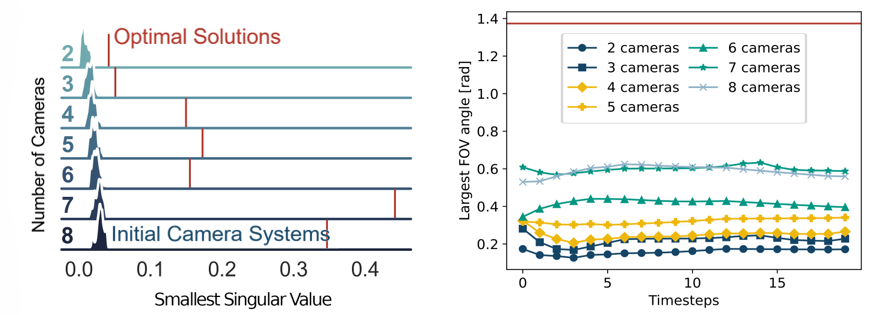
\includegraphics[width=\columnwidth]{graphics/fov_sv_conflict.png}
	\caption{The conflict between the field of view angle and the smallest singular value. Left: The smallest singular values of the system replicated from \cite{camera_placement}. Right: The largest angle of a marker to the optical axis.
		Comparing both one can see that lower singular values correlate with lower maximum field of view (FOV) angles.}
	\label{fig:fov_sv_conflict}
\end{figure}

It also has practical advantages.
Replicating the results of \cite{camera_placement} where the smallest singular value was used as a measure of the quality of the camera placement we can additionally plot the largest angle to the optical axis.
Here we see that the system always tries to find a trade off between minimizing the field of view angle while trying to maximize the smallest singular value.\\
This is shown in Fig.~\ref{fig:fov_sv_conflict}.
In a unified error description this problem does not exist and the system can be optimized for the best possible accuracy.



\section{Outlook}
experimental validation of measurement system
- Outlook, Planing Invertation
- Tradeoff



%\section{Online license transfer}
%All authors are required to complete the Procedia exclusive license transfer agreement before the article can be published, which they can do online. This transfer agreement enables Elsevier to protect the copyrighted material for the authors, but does not relinquish the authors’ proprietary rights. The copyright transfer covers the exclusive rights to reproduce and distribute the article, including reprints, photographic reproductions, microfilm or any other reproductions of similar nature and translations. Authors are responsible for obtaining from the copyright holder, the permission to reproduce any figures for which copyright exists.
%
%\vfill\pagebreak

\section*{Acknowledgements}
The authors would like to thank the Ministry of Science, Research and Arts of the Federal State of Baden-Württemberg for the financial support of the projects within the InnovationsCampus Future Mobility (ICM).


%% The Appendices part is started with the command \appendix;
%% appendix sections are then done as normal sections
%% \appendix

%% \section{}
%% \label{}

%\appendix
%\section{An example appendix}
%Authors including an appendix section should do so before References section. Multiple appendices should all have headings in the style used above. They will automatically be ordered A, B, C etc.


\bibliographystyle{elsarticle-harv}
\bibliography{sources}


%% Authors are advised to use a BibTeX database file for their reference list.
%% The provided style file elsarticle-num.bst formats references in the required Procedia style

%%%%%%%%%% If preparing manually:

%% For references without a BibTeX database:

% \begin{thebibliography}{00}
	
	%% \bibitem must have the following form:
	%%   \bibitem{key}...
	%%
	
	% \bibitem[Clark et al.(1962)]{clark}Clark, T., Woodley, R., De Halas, D., 1962. Gas-Graphite Systems, in ``{\it Nuclear Graphite}’’.
	% In: Nightingale, R. (Ed.). Academic Press, New York, pp. 387.
	
	% \bibitem[Deal and Grove(2009) ]{Deal}Deal, B., Grove, A., 1965. General Relationship for the Thermal Oxidation of Silicon. Journal of Applied Physics 36.2, 37--70.
	
	% \bibitem[Deep(2009)]{Deep}Deep-Burn Project: Annual Report for 2009, Idaho National Laboratory, Sept. 2009.
	
	% \bibitem[Fachinger(2004)]{Fachinger2004}Fachinger, J., den Exter, M., Grambow, B., Holgerson, S., Landesmann, C., Titov, M., Podruhzina, T., 2004. ``Behavior of spent HTR fuel elements in aquatic phases of repository host rock formations,’’ 2nd International Topical Meeting on High Temperature Reactor Technology. Beijing, China, paper \#B08.
	
	% \bibitem[Fachinger(2006)]{Fachinger2006}Fachinger, J., 2006. Behavior
	% of HTR Fuel Elements in Aquatic Phases of Repository Host Rock Formations. Nuclear Engineering \& Design 236.3,      54.
	
	% \end{thebibliography}

\clearpage\onecolumn

%%%% This page is for instructions only, once the article is finalize please omit the below text before creating the final PDF
\normalMode

%\section*{Instructions to Authors for LaTeX template:}
%
%\section{ZIP mode for LaTeX template:}
%
%The zip package is created as per the guide lines present on the URL http://www.elsevier.com/author-schemas/ preparing-crc-journal-articles-with-latex for creating the LaTeX zip file of Procedia LaTeX template.  The zip generally contains the following files:
%\begin{Itemize}[]\leftskip-12.7pt\labelsep3.3pt
%	\item ecrc.sty
%	\item  elsarticle.cls
%	\item elsdoc.pdf
%	\item .bst file
%	\item Manuscript templates for use with these bibliographic styles
%	\item  Generic and journal specific logos, etc.
%\end{Itemize}
%
%The LaTeX package is the main LaTeX template. All LaTeX support files are required for LaTeX pdf generation from the LaTeX template package.
%
%{\bf Reference style .bst file used for collaboration support:} In the LaTeX template packages of all Procedia titles a new ``.bst’’ file is used which supports collaborations downloaded from the path http://www.elsevier.com/author-schemas/the-elsarticle-latex-document-class

\end{document}

%%
%% End of file.
